\chapter{Conception}
\label{chap:conception}
\section{Introduction}
\section{Identified Gaps and Proposed Solution Overview}
\section{Global Architecture of the Framework}
\section{Detection Models}
\label{sec:detection-models}
\subsection{Autoencoder}
\subsection{VAE}
\subsection{Transformer}
\subsection{GNN}
\section{Synthetic Data Augmentation with Generative AI}
\label{sec:synthetic-data}
\subsection{Motivation}
\subsection{REaLTabFormer}
\subsection{Timestamp Generation}
\subsection{Validation Strategy}
\section{Reinforcement Learning Agent}
\label{sec:rl-agent}
\subsection{Architecture and role}
\subsection{Training process}
\subsection{Ablation Study}
\section{Platform Architecture and Design}
\label{sec:platform-design}

% --- 1. Set the scene -------------------------------------------------
\subsection{Overview of the Platform}
\label{sec:platform-overview}

This section introduces CAVIX, the platform that assembles the
detector of section~\ref{sec:detection-models}, the synthetic
generator that augments scarce attack stages
(section~\ref{sec:synthetic-data}), and the reinforcement-learning
response agent (section~\ref{sec:rl-agent}) into a single system an
analyst can run, observe, and trust. A platform here is more than the
collection of models: it is the engineering surface around them,
namely ingestion of real Wazuh alerts \cite{wazuh2024}, a message
bus decoupling slow inference from fast collection, a persistence
layer recording every verdict for forensic review, threat-intelligence
enrichment, and analyst-facing web and mobile applications. We
present it through four architectural concerns: structure, behaviour,
data, and deployment.

Three design goals drive the platform. Reproducibility means that a
replayed alert yields the same verdict on a fixed configuration.
Component replaceability means that the SIEM, the bus, the database,
the feeds, and the front-ends sit behind narrow contracts, so that
any one can be swapped through its adapter. Type-safe contracts
end-to-end mean that a single schema validates backend alerts and
generates the client types. Each goal answers a concrete APT
requirement: re-investigating weeks-long attack chains, surviving
heterogeneous SOCs, and keeping multi-stage investigations consistent
across devices.

\paragraph{Trust assumptions.} The adversary controls the attacker
zone and may compromise individual hosts. The Wazuh manager, the
model registry (content-hashed), and the inference workers are
trusted; stronger threat models are out of scope.

% --- 2. Static structure: from the big picture down to the code -------
\subsection{System Architecture Diagram}
\label{sec:platform-arch}

The platform is organised as five logical layers, drawn in
figure~\ref{fig:ch3:archcomp}. Each layer has one responsibility and
communicates with the next only through a documented contract.

\begin{figure}[H]
  \centering
  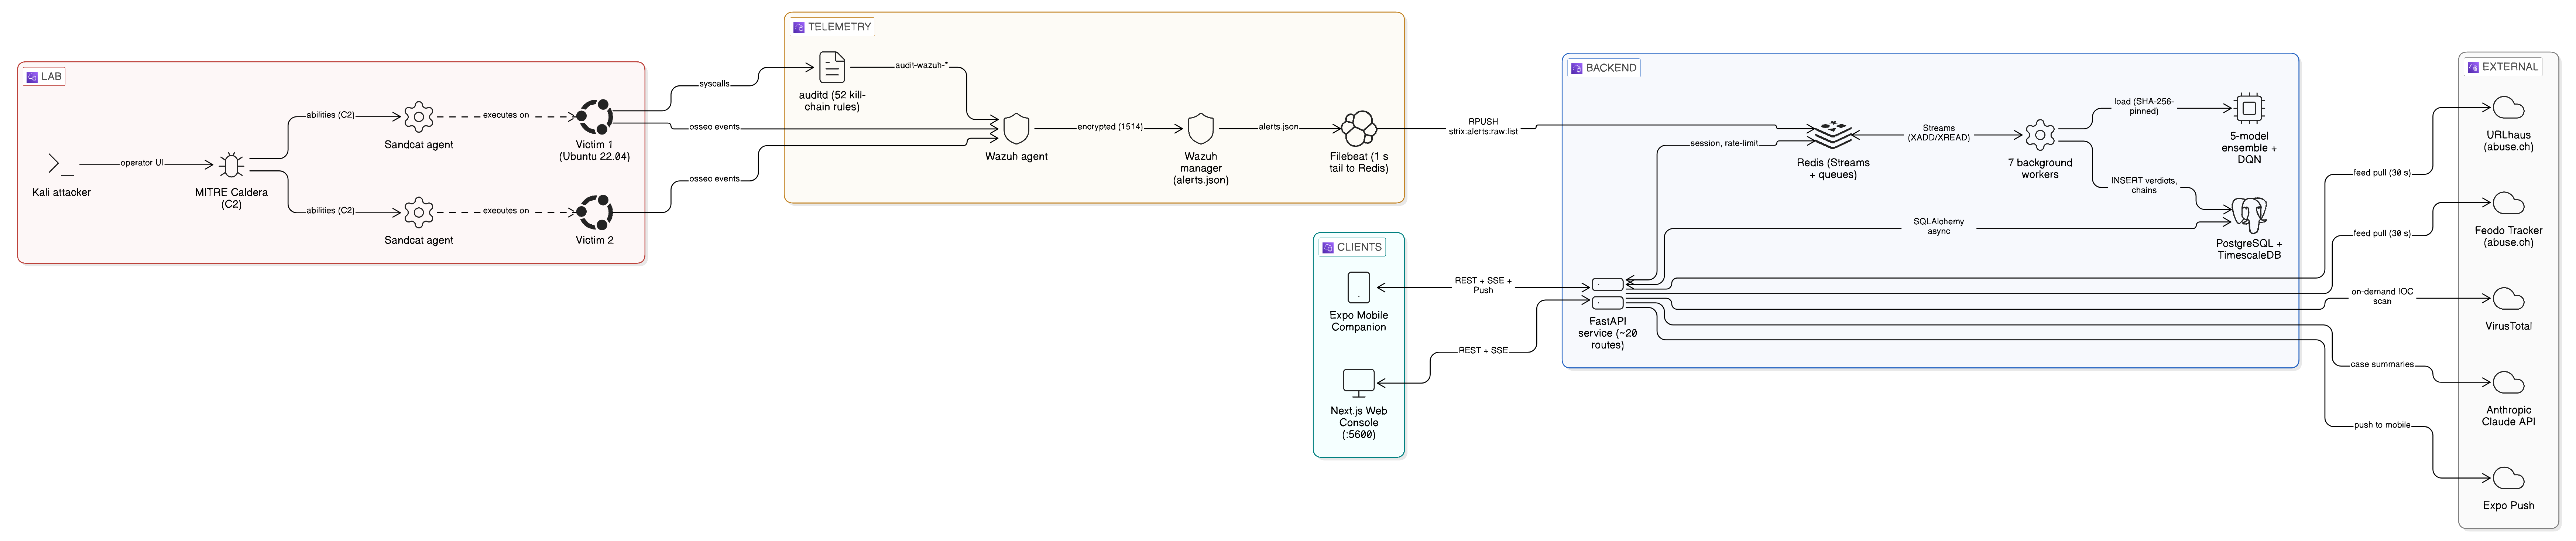
\includegraphics[width=0.95\textwidth]{figures/ch3/eraser/system-arch-diagram}
  \caption{Logical architecture of the CAVIX platform.}
  \label{fig:ch3:archcomp}
  \par\medskip
  As figure~\ref{fig:ch3:archcomp} shows, the five layers (sensing, transport, intelligence, persistence, and presentation) are stacked vertically; arrows indicate the direction in which data flows. The dashed envelope around the intelligence layer marks the boundary inside which the conceptual framework of sections~\ref{sec:detection-models}--\ref{sec:rl-agent} operates.
\end{figure}

The \textbf{sensing layer} converts host activity into structured
events. It combines the Linux audit subsystem
\cite{auditd2024}, which exposes kernel syscalls of interest, and a
Wazuh agent on each monitored host, which forwards the resulting
alerts to a Wazuh manager. The manager applies the custom rule
hierarchy described later in chapter~\ref{chap:implementation} and
writes one JSON line per alert to a local file. From the platform's
point of view, that file is the only contract with the SIEM.

The \textbf{transport layer} moves alerts from the sensing layer into
the rest of the platform. It uses a log-shipper to tail the alert file
\cite{filebeat2024} and a stream-based message bus \cite{redis2024} as
the durable backbone between workers. The stream-based design is a
deliberate departure from synchronous remote-procedure calls: it
absorbs ingestion bursts, decouples the producer's pace from the
consumer's, and provides at-least-once semantics that make replay
during evaluation straightforward.

The \textbf{intelligence layer} is where the conceptual framework of
the earlier sections runs. It hosts the normaliser that
materialises the 55-dimensional feature vector, the inference worker
that hosts the four detection models of section~\ref{sec:detection-models},
the reinforcement-learning policy of section~\ref{sec:rl-agent}, and
the deterministic gate that wraps the RL action. The intelligence
layer never reads from or writes to the SIEM; it only consumes a
feature stream and emits a verdict stream.

The \textbf{persistence layer} records verdicts and the entities derived
from them: hosts, alerts, attack chains, DQN actions, and threat
indicators. We use a relational store \cite{postgres2024} extended for
time-series workloads \cite{timescaledb2024}, because the dominant
query pattern is "give me everything for host~$h$ in the last
$\Delta t$ minutes", which time-partitioned tables answer
efficiently. The schema is described in section~\ref{sec:class-diagram}.

The \textbf{presentation layer} comprises the analyst-facing web
console \cite{nextjs2024} and the mobile companion \cite{expo2024}.
Both clients consume the same OpenAPI specification, which makes the
backend the single source of truth for what an alert, a verdict, or a
chain looks like. A server-sent-events channel pushes new verdicts to
the web console; the mobile client receives push notifications for
early-stage detections only, to avoid alert fatigue.

\subsection{Platform Components}
\label{sec:platform-components}

This subsection examines the four components that an analyst
interacts with directly. The transport and persistence layers are
treated as plumbing and are not detailed individually; the data-flow
view of section~\ref{sec:dataflow} covers them.
Figure~\ref{fig:ch3:components} situates the four components and
their inputs and outputs inside the layered architecture of
figure~\ref{fig:ch3:archcomp}.

\begin{figure}[H]
  \centering
  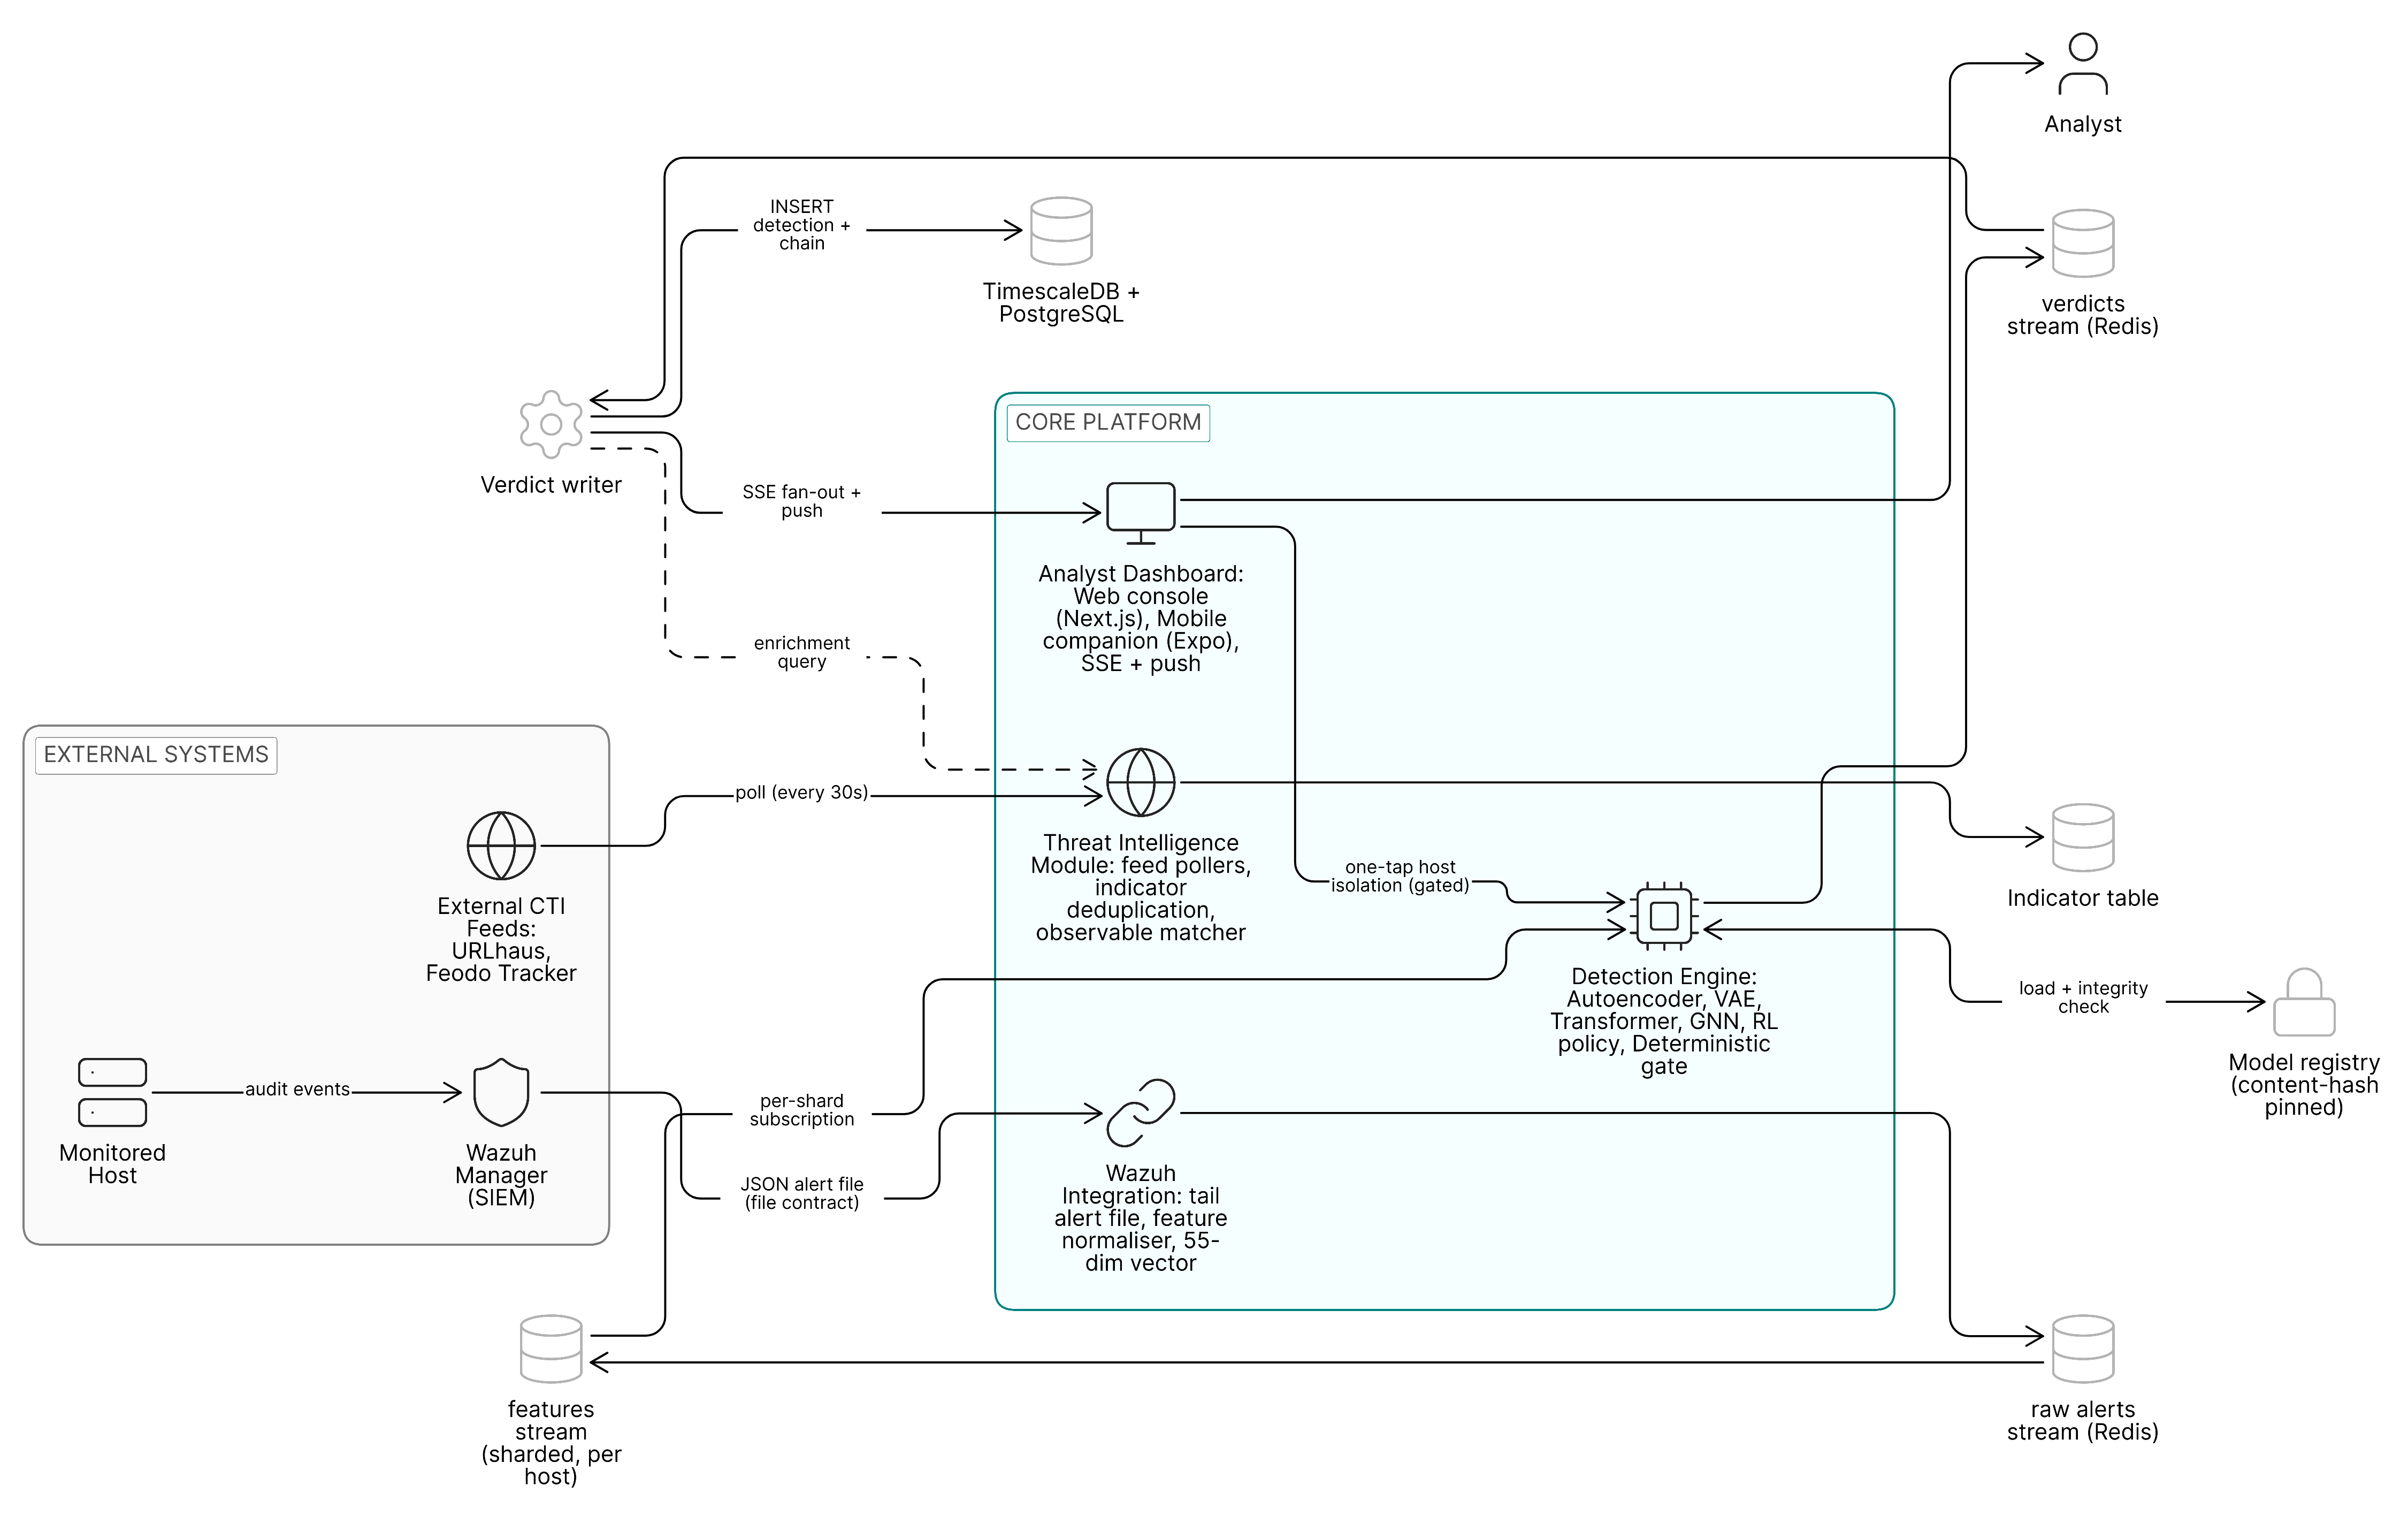
\includegraphics[width=0.95\textwidth]{figures/ch3/eraser/platform_components_v2}
  \caption{Platform components view of CAVIX.}
  \label{fig:ch3:components}
  \par\medskip
  As shown in figure~\ref{fig:ch3:components}, the four analyst-facing components (Wazuh Integration, Detection Engine, Threat Intelligence Module, and Analyst Dashboard) are grouped in the teal Core Platform cluster, with their inbound and outbound contracts shown explicitly; the transport streams, persistence stores, and model registry appear in light gray as the plumbing the components read from and write to. External systems (Wazuh manager, CTI feeds, monitored host) sit on the left; the analyst is on the right.
\end{figure}

\subsubsection{Detection Engine}

The detection engine is the only component that hosts model weights.
It runs as a pool of inference workers, each subscribed to one shard
of the feature stream, and is responsible for three operations: loading
the model artefacts on startup, batching incoming feature vectors,
and emitting a verdict on the verdict stream. The four detection
models of section~\ref{sec:detection-models} and the RL policy of
section~\ref{sec:rl-agent} are loaded as ordinary tensor modules; the
deterministic gate that wraps the RL action is implemented as a
post-processing step inside the same worker, so that no intervention
action can leave the engine without passing through it.

Two design decisions matter at this level. The engine validates the
integrity of every artefact it loads against a registry that pins each
weight by content hash; an artefact whose hash drifts away from the
registry refuses to load. This is the mechanism that enforces the
reproducibility goal of section~\ref{sec:platform-overview}. The
engine also batches inference: the worker collects up to a fixed
number of events from its shard before invoking the models, which
amortises the per-batch fixed cost over many alerts. Both decisions
trade a small amount of latency for a substantial gain in stability,
which we judge appropriate for a platform whose verdicts have to be
defensible after the fact.

The deterministic gate inside the engine is conceptually simple and
its concrete thresholds are deferred to chapter~\ref{chap:implementation}.
An intervention proposed by the RL policy
(\texttt{ESCALATE}, \texttt{ISOLATE\_HOST}, or \texttt{BLOCK\_USER\_IP})
is authorised only when all four detection-side scores
(autoencoder reconstruction error, VAE anomaly probability,
Transformer confidence on the predicted kill-chain stage, and GNN
per-node risk) cross their respective thresholds. A single check
that fails downgrades the action to \texttt{LOW\_ALERT}, leaving the
analyst the option to intervene manually. This conjunctive gating
is the architectural reflection of a conservative bias: the platform
refuses to act on the RL policy alone, and an intervention requires
the agreement of every detection model.

\subsubsection{Wazuh Integration}

The Wazuh integration is intentionally thin. We do not patch the Wazuh
manager binary and we do not embed Wazuh logic inside the platform.
The integration consists of three artefacts maintained on the SIEM
side (a set of audit rules tuned for the Linux kill chain
\cite{auditd2024}, a custom rule file installed in the manager's
configuration, and a muting hierarchy that silences noisy parent rules
in favour of a small number of high-value child rules) and one
contract on the platform side, namely the alert file that the manager
writes. Treating Wazuh as a black box behind a file contract keeps
the SIEM swappable later and matches how real SOCs operate, in which
the SIEM is rarely a component the analyst team owns end-to-end. The price of this design is an explicit trust
assumption: the platform treats the manager's alert file as its
ground truth of host activity. A compromised manager could silently
omit alerts or rewrite rule matches, and the intelligence layer would
have no way to detect it. We accept this assumption in the scope of
this thesis on the same grounds a SOC accepts it in practice: the
SIEM is hardened separately, the platform does not extend the attack
surface of the manager, and the manager's integrity is the analyst
team's concern, not the detection layer's.

\subsubsection{Threat Intelligence Module}

The threat-intelligence module enriches internal verdicts with
external context. It periodically polls two open-source feeds
\cite{urlhaus2024,feodotracker2024}, deduplicates indicators by
\texttt{(value, type, source)}, and stores them in a single indicator
table. When a verdict is persisted, the verdict-writer queries that
table to flag any observable in the alert (IP, URL, domain, file
hash) that intersects an indicator; the resulting "observable hit"
becomes a feature in the chain forensic view exposed by the dashboard.

The module is deliberately feed-agnostic. Adding a new feed is a
single function that returns a list of indicator dictionaries;
everything else (the polling cadence, the deduplication, the
circuit-breaker protecting the feed call, and the staleness badge in
the UI when a feed is degraded) is generic. Here the component-replaceability
goal has a concrete payoff: a new public or commercial feed can be
plugged in without touching any other layer.

\subsubsection{Analyst Dashboard}

The dashboard turns the platform into a tool an analyst can operate.
It exposes four primary views: a model-monitoring view that surfaces the
live anomaly scores and class probabilities of the ensemble; an
attack-analysis view that reconstructs attack chains by grouping
consecutive alerts from the same host and matching them against the
nine MITRE-aligned tactics \cite{mitre_attack}; a topology view that
plots the live simulation graph against the GNN's per-node risk
score; and a threat-intelligence view that surfaces the most recent
observable hits.

The mobile companion is a deliberate subset of the web functionality,
not a parallel reimplementation. It exposes the vigilance feed of
verdicts, a chain detail page, and a one-tap host-isolation control
that re-uses the same gated endpoint as the web console. Both
clients are generated from the same OpenAPI types; a breaking change
to the backend therefore fails the client build before it can reach
an analyst's screen.

\subsection{Class Diagram}
\label{sec:class-diagram}

The backend domain model contains six load-bearing entities,
small enough to summarise on a single diagram.
Figure~\ref{fig:ch3:classdiag} shows these entities and their
relationships.

\begin{figure}[H]
  \centering
  \includegraphics[width=0.95\textwidth,height=0.78\textheight,keepaspectratio]{figures/ch3/eraser/class-diagram}
  \caption{UML class diagram of the backend domain model.}
  \label{fig:ch3:classdiag}
  \par\medskip
  In figure~\ref{fig:ch3:classdiag}, solid edges are persisted foreign-key relationships. \texttt{Alert} and \texttt{Detection} are TimescaleDB hypertables (composite primary key on \texttt{alert\_id}, \texttt{occurred\_at}); every other entity is an ordinary relational table.
\end{figure}

A \texttt{Host} represents one monitored machine, identified by its
Wazuh agent identifier; it has a current risk score, last-seen
timestamp, and inventory metadata. An \texttt{Alert} represents one
Wazuh JSON line and carries the raw observables; it is referenced by
exactly one \texttt{Detection}, which records the five model outputs
(four anomaly scores plus the gated RL action) and the kill-chain
stage. The stage is one of the nine MITRE ATT\&CK tactics covered by
the Linux APT Dataset 2024 \cite{mitre_attack}, projected onto the
seven-stage Cyber Kill Chain as defined in
chapter~\ref{chap:implementation}; the same nine-tactic taxonomy
drives the topology view of the analyst dashboard and the dataset
sampling described in chapter~\ref{chap:implementation}.

An \texttt{AttackChain} groups consecutive detections from the same
host into a single investigation thread; the grouping window is a
configuration parameter, not a hard-coded constant. This entity is
the architectural feature that makes the platform APT-aware. The
defining property of an Advanced Persistent Threat is that it spans
many low-signal events across multiple kill-chain stages over an
extended dwell time, so a detection layer that surfaces alerts
individually is operationally blind to the chain itself. The
\texttt{AttackChain} entity gives the analyst a unit of investigation
matched to the adversary's unit of action, and it gives the RL agent
of section~\ref{sec:rl-agent} the temporal scope over which an
escalating intervention is justified rather than reflexive.

A \texttt{DQNAction} records the action that survived the
deterministic gate, together with the four threshold checks that
authorised it; the action history is the audit trail an analyst
consults when a post-mortem asks why the platform intervened. An
\texttt{IntelIndicator} is one row from a CTI feed and is associated
with the detections it enriches; the association is computed at
write time, so adding a new feed does not require backfilling.

On the service side, four worker classes mirror the five-stage pipeline
of section~\ref{sec:dataflow}: the \texttt{WazuhBridge} drains the
log-shipper's staging buffer, the \texttt{Normalizer} produces the
feature vector, the \texttt{InferenceWorker} hosts the models and the
RL gate, and the \texttt{VerdictWriter} persists results and fans them
out over server-sent events and push notifications. The
\texttt{IntelFeedsWorker} runs on its own schedule and is the only
worker not driven by the pipeline.

% --- 3. Dynamic behaviour: coarsest to finest -------------------------
\subsection{Workflow Diagram}
\label{sec:workflow}

Figure~\ref{fig:ch3:workflow} traces a single alert through the
platform, from the moment Wazuh writes the JSON line until the verdict
appears on the analyst's screen.

\begin{figure}[H]
  \centering
  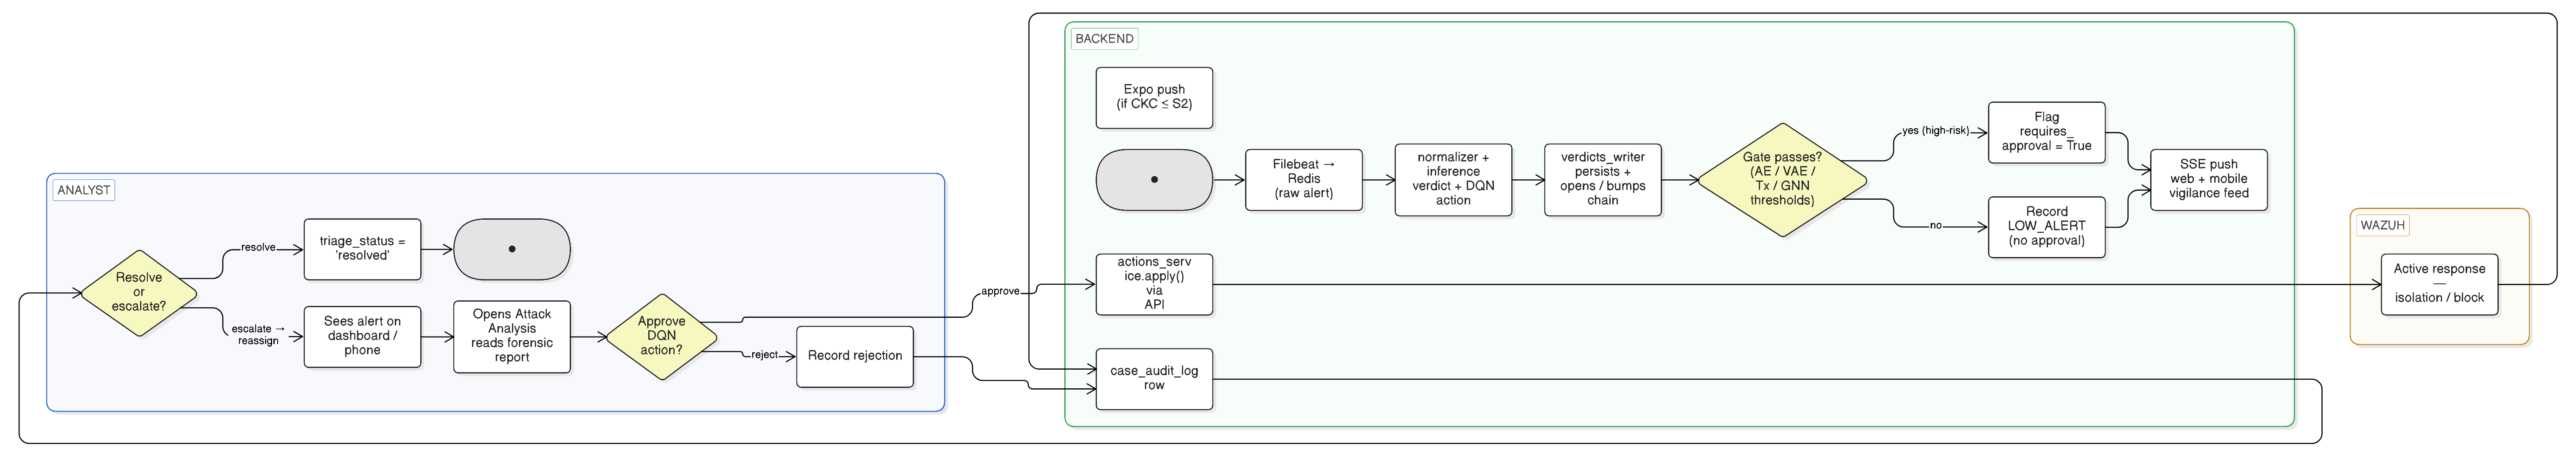
\includegraphics[width=0.95\textwidth]{figures/ch3/eraser/workflow-diagram}
  \caption{End-to-end analyst-response workflow.}
  \label{fig:ch3:workflow}
  \par\medskip
  As illustrated in figure~\ref{fig:ch3:workflow}, swim-lanes group activities by actor (backend pipeline, analyst, Wazuh active response); diamonds are decision points. Everything inside the backend lane is replayable from the feature vector, which is why the evaluation chapter can rerun historical alerts without touching the SIEM.
\end{figure}

The workflow is decomposed into seven activities. \emph{Ingestion}
turns the alert file into messages on the raw stream. \emph{Feature
construction} parses the alert, looks up the host, runs the SecBERT
embedding plus PCA reduction described in
section~\ref{sec:detection-models}, and writes the 55-dimensional
feature vector to the feature stream. \emph{Ensemble inference}
runs the four detection models on a batch of vectors and assembles
the thirteen-dimensional state vector that the RL policy consumes.
\emph{RL decision} produces an action proposal (monitor, low alert,
escalate, isolate host, or block user--IP). \emph{Deterministic
gating} accepts or downgrades that action based on four threshold
checks against the anomaly scores; this is the step that ensures a
single high-confidence model is required for any intervention.
\emph{Persistence} writes the alert, the detection, the optional DQN
action, and updates the open attack chain. \emph{Fan-out} pushes the
verdict over the server-sent-events channel to the web console and,
for early-stage detections, sends a push notification to the mobile
client.

The activities are loosely coupled. Each one consumes from an
upstream stream or table and emits to a downstream one; no activity
holds state between alerts beyond the model weights it loaded at
startup. This statelessness allows the intelligence layer to be
replayed deterministically: feeding the same feature vectors
in the same order reconstructs the same verdicts, which is the
property the evaluation chapter relies on to compute model-level
metrics offline.

\subsection{Data Flow Design}
\label{sec:dataflow}

The data flow concretises the workflow as a sequence of stream
transitions. Three principles shape its design.

First, every transition between two workers goes through a named
stream with a documented message schema, never through a direct
function call. This converts the platform from a monolithic Python
process into a set of independent processes that can be restarted,
profiled, and scaled in isolation. The price is one serialisation
hop per stage; the benefit is a clean failure boundary, since a
crash in the inference worker no longer corrupts the alert that the
normaliser is currently processing.

Second, feature messages are sharded by host. The shard key is a
hash of the agent identifier modulo the configured shard count, which
gives the platform deterministic affinity (every alert from
host~$h$ lands on the same inference worker) without any explicit
routing logic. Affinity matters because the GNN of
section~\ref{sec:detection-models} consumes a victim graph whose
features benefit from temporal locality: keeping a host's alerts on
the same worker amortises the cost of refreshing the local
neighbourhood the GNN reasons over, instead of paying the rebuild
cost on every shard reassignment. Hash-modulo routing also creates
the possibility of skew when a single noisy host dominates the
traffic of one shard, an effect the deployment posture of
section~\ref{sec:deployment} accepts on the single-host evaluation
topology.

Third, every message schema is a versioned data class with a hash
of its definition pinned in the message envelope. A producer that
emits an older schema version is rejected by the consumer, rather
than being silently coerced into the current format. We adopted this
discipline after an early prototype produced a subtle off-by-one in
the kill-chain stage field that survived all unit tests because the
test fixtures had drifted away from the production schema.

\paragraph{Stream layout.} The platform uses five logical streams.
A staging buffer between the log-shipper and the bridge worker; a
\emph{raw alerts} stream between the bridge and the normaliser; a
sharded \emph{features} stream between the normaliser and the
inference workers; a single \emph{verdicts} stream between the
inference workers and the verdict writer; and a server-sent-events
broadcast channel between the verdict writer and the dashboards.
Only the staging buffer and the broadcast channel are bounded; the
three internal streams are durable so that a crashing worker can
resume from its last committed offset without losing in-flight
messages.

\subsection{Sequence Diagram}
\label{sec:sequence}

Figure~\ref{fig:ch3:sequence} captures the timed interaction between
the actors involved in a single early-stage APT detection event,
specifically the moment when a Reconnaissance burst against an
exposed SSH service produces the first verdict of an attack chain.

\begin{figure}[H]
  \centering
  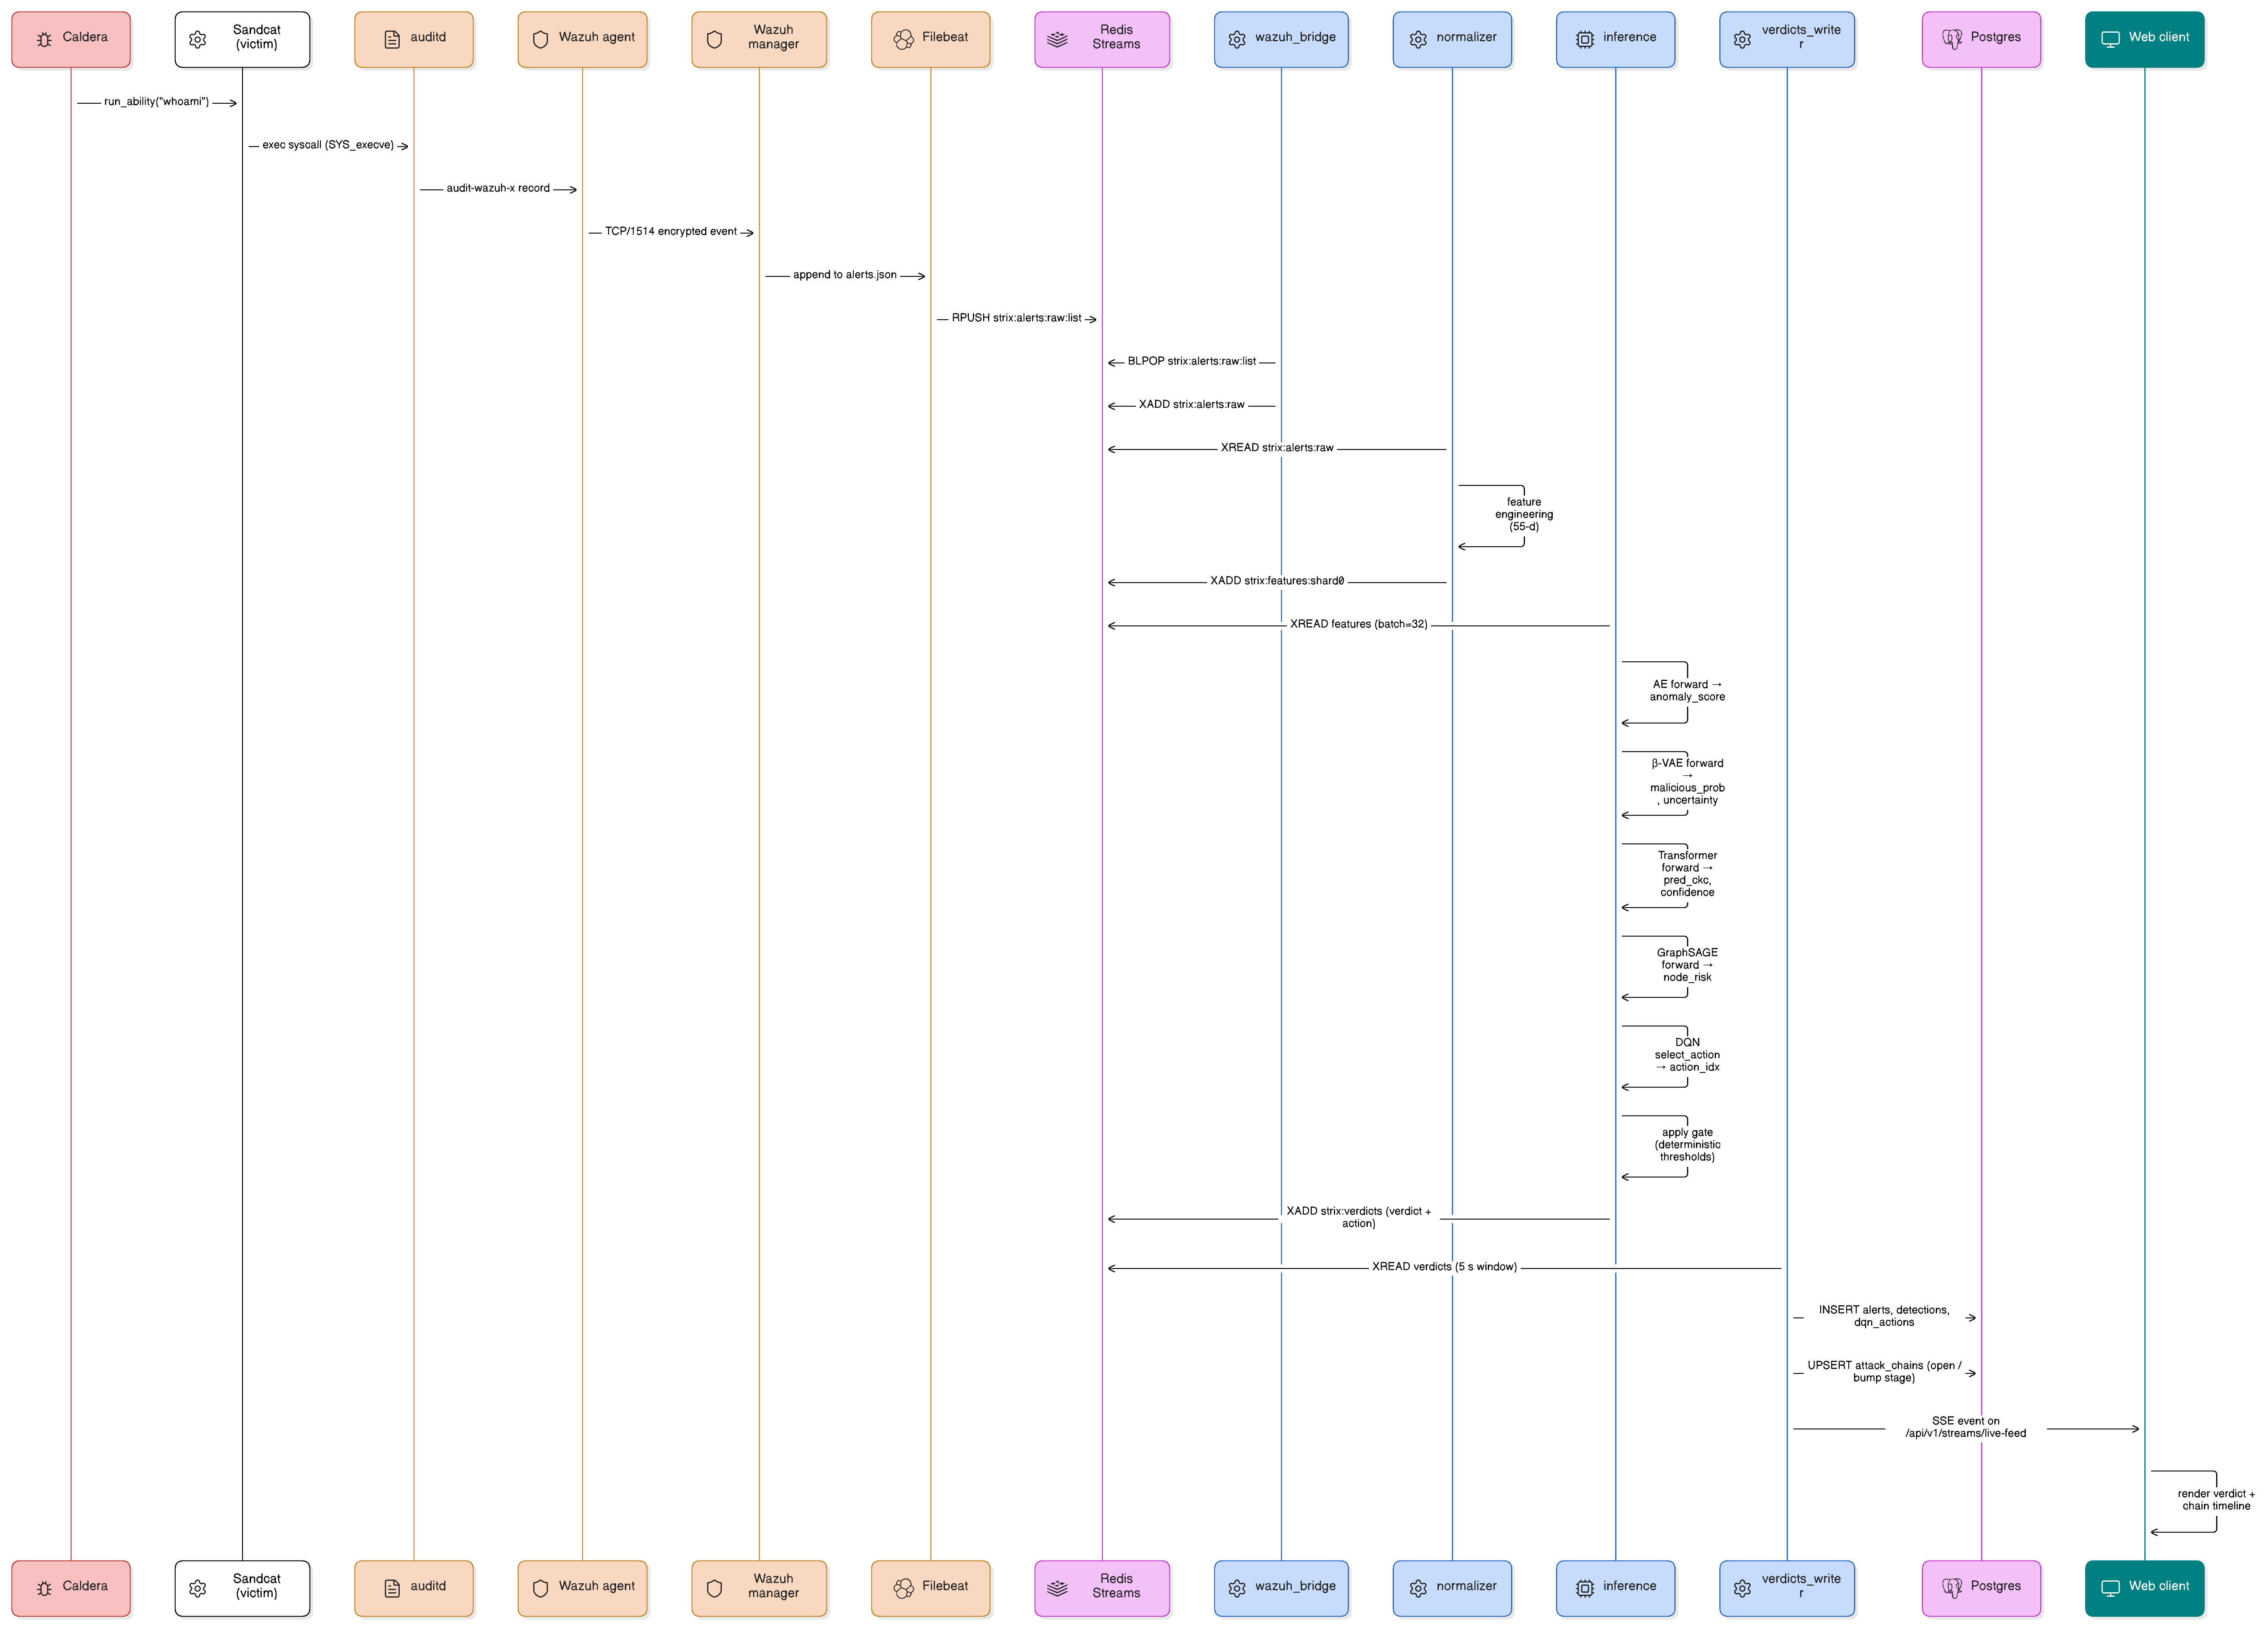
\includegraphics[width=0.95\textwidth]{figures/ch3/eraser/sequence-diagram}
  \caption{Sequence diagram for a single early-stage detection event.}
  \label{fig:ch3:sequence}
  \par\medskip
  As depicted in figure~\ref{fig:ch3:sequence}, vertical bars are participants; horizontal arrows are messages. Time flows downward. The self-loops on the inference worker are the synchronous calls into each detection model, the RL policy, and the deterministic gate that is evaluated before any verdict is emitted.
\end{figure}

The scenario unfolds as follows. The attacker host issues a burst of
\texttt{sshd} authentication probes against a victim. The victim's
audit subsystem records each \texttt{execve} of the SSH daemon's
worker; the Wazuh agent forwards the corresponding rule match to the
manager, which appends a JSON alert to its alert file. The
log-shipper detects the new line within its check interval and
pushes it into the staging buffer.

The bridge worker dequeues the line and writes it to the raw stream;
the normaliser reads it, performs the feature transformation, and
publishes the feature vector on the appropriate shard of the feature
stream. The inference worker subscribed to that shard runs the
ensemble synchronously, derives the state vector, queries the RL
policy, and emits a verdict on the verdict stream. The verdict
writer evaluates the deterministic gate against the four anomaly
scores: in this scenario the autoencoder and the GNN both report
above-threshold values, so the proposed \texttt{ESCALATE} action is
authorised. The writer persists the detection and opens a new attack
chain, broadcasts the verdict over server-sent events, and triggers
a push notification to the analyst's mobile client because the
kill-chain stage is S1.

The diagram makes one architectural commitment visible: no worker on
the detection pipeline blocks on a synchronous remote-procedure call
to any other worker. All cross-process communication along the
pipeline is mediated by streams or by the database, while the
dashboard and the mobile push gateway sit downstream of the verdict
writer on a fan-out channel. A failure of the dashboard, the mobile
push gateway, or any single inference worker therefore degrades the
platform gracefully rather than stalling the detection pipeline.

% --- 4. Where it physically runs --------------------------------------
\subsection{Deployment Architecture}
\label{sec:deployment}

Figure~\ref{fig:ch3:deploy} shows the deployment topology used in the
defence lab and in the evaluation of chapter~\ref{chap:evaluation}.

\begin{figure}[H]
  \centering
  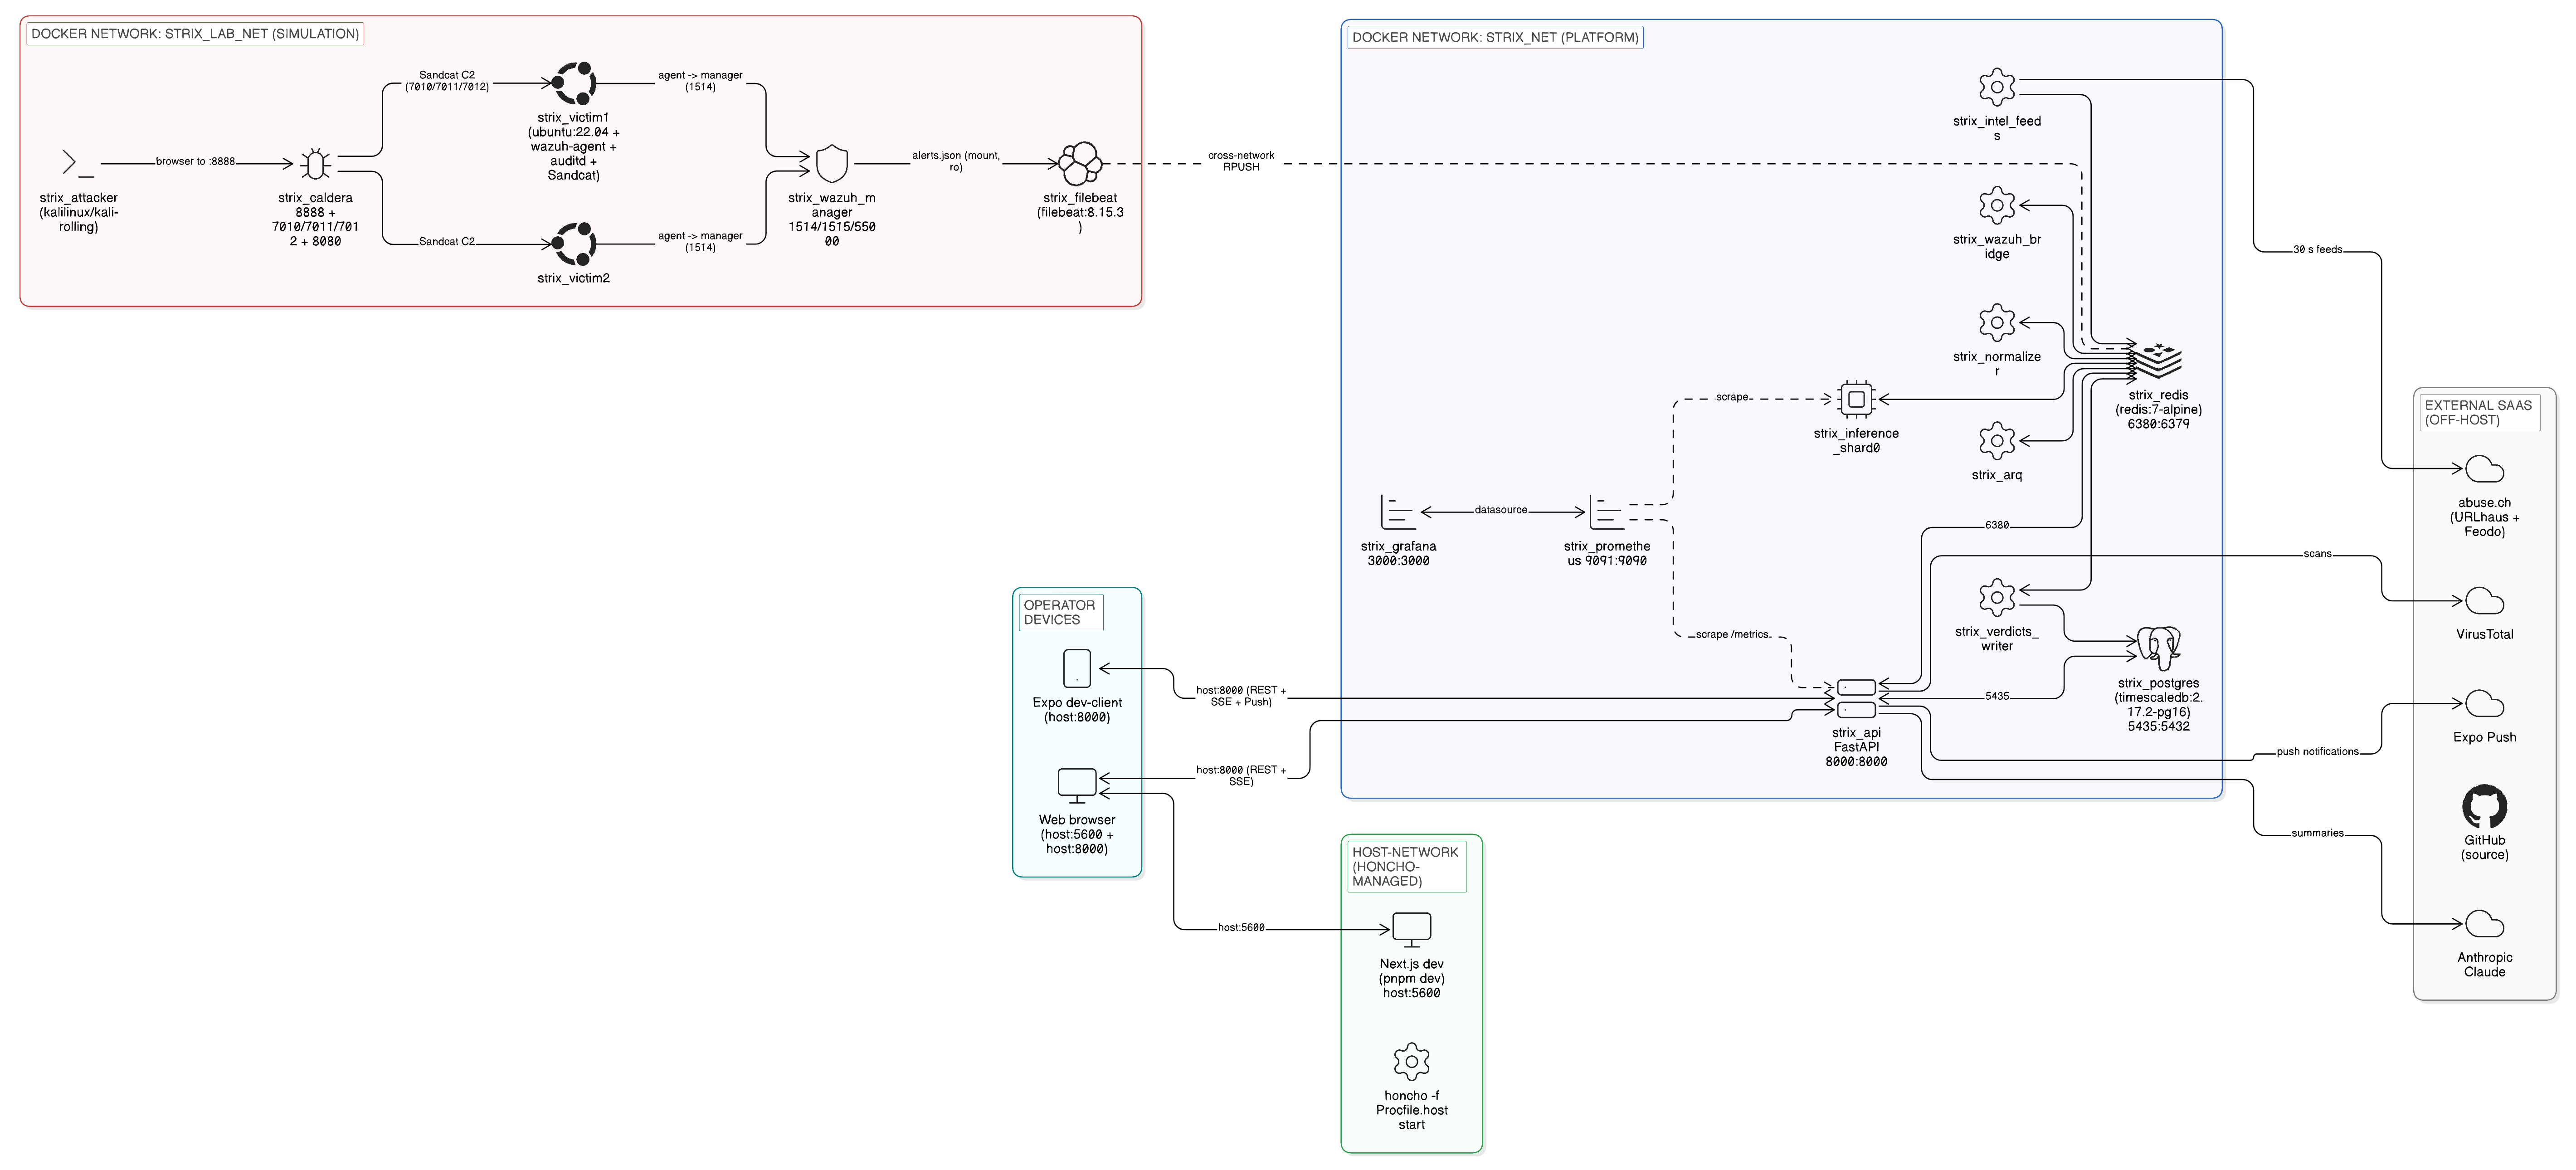
\includegraphics[width=0.95\textwidth]{figures/ch3/eraser/deployment-diagram}
  \caption{Deployment topology.}
  \label{fig:ch3:deploy}
  \par\medskip
  As figure~\ref{fig:ch3:deploy} shows, every component runs in a container \protect\cite{docker2024} on a shared bridge network. The attacker, victims, SIEM, and platform services are grouped into four logical zones; inter-zone traffic is restricted by the bridge's firewall rules, while intra-zone traffic is unrestricted so that the attacker can reach the victims directly.
\end{figure}

Four logical zones structure the topology. The \emph{attacker zone}
hosts a Kali container running the MITRE Caldera command-and-control
server \cite{caldera2024}, which drives the attack scenarios used
during evaluation. The \emph{victim zone} hosts the two Ubuntu
containers under observation; each one carries an audit subsystem, a
Wazuh agent, and a Caldera Sandcat implant that lets the attacker
zone deliver abilities. The \emph{SIEM zone} hosts the Wazuh manager,
the log-shipper, and the staging buffer; nothing else writes to the
buffer, which keeps the contract between sensing and platform clean.
The \emph{platform zone} hosts the relational store, the bridge, the
normaliser, the inference worker, the verdict writer, the intel
feeds worker, the API gateway, and the web console.

The topology has two deployment postures. The \emph{single-host
lab} posture, used throughout this thesis, runs every container on
one workstation; this is sufficient for development, for the jury
demonstration, and for the evaluation in chapter~\ref{chap:evaluation},
because the alert volumes generated by Caldera in the nine-tactic
scenario fit comfortably inside a sixteen-gigabyte machine without a
GPU. The \emph{distributed posture}, which we describe but do not
exercise, places the SIEM and the victim hosts on physical or virtual
machines, retains the platform services as a container stack on a
separate host, and adds horizontal scaling of inference workers
behind the sharded feature stream. The transition from one posture to
the other does not require code changes; it requires only the
configuration of inter-host network reachability and the matching
adjustment of the shard count.

A note on operational concerns. Persistent state (the relational
database, the threat-indicator table, the model registry, and the
Caldera operations directory) is mounted from the host into the
relevant containers, so that a rebuild does not destroy historical
data. The mobile companion runs on a real device or emulator outside
the bridge network and reaches the platform through the API gateway
\cite{expo2024,nextjs2024}; this is the only inbound connection
crossing the bridge boundary, which simplifies the security posture
of the deployment.
\section{Conclusion}
